
\chapter{Аналитический раздел}

В данном разделе будут представлены обзор предметной области, существующих методов определения позы человека, а также проведен сравнительный анализ этих методов.

\section{Обзор предметной области}

\subsection{Классические подходы к определению позы человека}

Глубокое обучение --- тип машинного обучения \cite{vyugin}, в котором используются искусственные нейронные сети с несколькими слоями для обработки сложных данных, которые активно используются в настоящее время в определении позы человека. Однако до его внедрения использовались другие методы, а именно: 
\begin{enumerate}[label=\arabic*)]
 	\item Модель пиктографических структур \cite{polygraphic}:
 	
 		Эта структура моделирует пространственные взаимосвязи частей твердого тела, выражая их в виде древовидной графической модели, чтобы предсказать местоположение суставов тела. 
 		Эти пространственные связи показаны с помощью пружин, и части представляют собой шаблоны внешнего вида, основанные на изображении. 
 		Путем параметризации частей с помощью расположения и ориентации пикселей, полученная структура может моделировать артикуляции. 
 		
 		На рисунке \ref{img:polygraphic} продемонстрировано наглядное представление этой модели.
 		\begin{figure}[ht!]
 			\centering
 			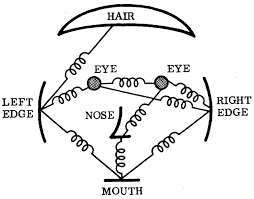
\includegraphics[width=0.4\linewidth]{assets/poly.png}
 			\caption{Пример пиктографической структуры.}
 			\label{img:polygraphic}
 		\end{figure}
 		
 		
 		Проблема этого подхода заключается в том, что он не может уловить корреляции между невидимыми и деформируемыми частями тела, что означает, что модель подвержена ошибкам, если не все конечности человека видны. 
 		Она также не зависит от данных изображения.
 		

 	\item Гибкое смешение частей \cite{FPE}:
 		
 		\begin{itemize}
 			\item Этот подход использует деформируемые модели частей, которые представляют собой коллекцию шаблонов, которые подбираются по изображению и располагаются в деформируемой конфигурации. 
 			Кроме того, каждая модель имеет глобальные шаблоны и шаблоны деталей. 
 			Основная идея заключается в том, чтобы использовать смесь мелких неориентированных деталей в отличие от использования семейства деформированных, то есть повернутых и ракурсных шаблонов.
 			Причина этого заключается в том, что с различиями в том, как выглядят конечности, и изменениями в точке зрения.
 			
 			\item Гибкое смещение частей одновременно фиксирует пространственные отношения между расположением деталей и отношения совпадения между смесями деталей, что приводит к моделям пиктографического структуры, которые кодируют исключительно пространственные отношения. 
 			Благодаря динамическому программированию, модели разделяют вычисления между аналогичными искривлениями, что делает этот подход не только значительно быстрым, но и высокоэффективным.
 			Кроме того они моделируют экспоненциально большой набор глобальных смесей через композицию смесей локальных частей для того, чтобы изучить понятия локальной жесткости, а также уловить влияние глобальной геометрии на локальный внешний вид, то есть внешний вид деталей различается в разных местах. 
 			На рисунке \ref{img:fpe} демонстрируется визуальное представление этой модели.
 			
 			\begin{figure}[ht!]
 				\centering
 				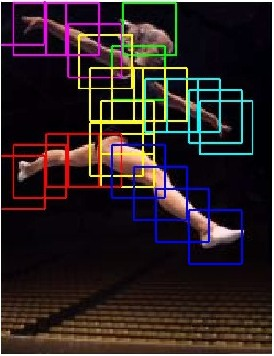
\includegraphics[width=0.3\linewidth]{assets/fpe.jpeg}
 				\caption{Пример гибкого смещения частей.}
 				\label{img:fpe}
 			\end{figure}
 			
 			\item Гибкое смещение частей способна хорошо выражать сложные отношения между суставами, поэтому она также может моделировать артикуляцию.
 			Однако у нее есть свои проблемы, которые включат ограниченную выразительность и отсутствие учета глобального контекста.
 			
 				
 		\end{itemize}
 		
 		
 	\item Края, цветочные гистограммы, контуры и гистограмма ориентированных градиентов были альтернативными характеристиками, которые применялись в ранних работах определения позы человека и служили основными строительными блоками различных классических моделей для определения точного местоположения частей тела \cite{polygraphic}. 
\end{enumerate}

К общим проблемам классических подходов относятся плохое обобщение и неточное обнаружение частей тела. Поэтому для решения этих проблем было применено глубокое обучение.

\section{Глубокое обучение в сверточных нейронных сетях в машине позирования}

Машина позирования состоит из последовательных мультиклассовых предсказаний, которых обучены предсказывать местоположение каждой детали на каждом уровне иерархии. Она также имеет модуль вычисления характеристик изображения и модуль предсказания, оба из которых могут быть заменены сверточной архитектурой \cite{CNN}, что позволяет позволяет изучать как изображения, так и контекстуальные представления признаков из данных.
Именно эта идея привела к созданию Convolutional Pose Machine (CPM), которая является первой моделью оценки позы человека на основе глубокого обучения \cite{wei2016cpm}.

CPM полностью дифференцируема, что позволяет обучать ее многоступенчатую архитектуру по принципу обратного распространения, алгоритму, используемому для обучения нейронных сетей с прямой передачей 
Кроме того, ее последовательная структура предсказания, состоящая из сверточных сетей и обучается неявным пространственным моделям, использует большие рецепторные поля на картах доверия, полученных на предыдущих этапах, что помогает в изучении пространственных связей между деталями на большом расстоянии и приводит к повышению точности за счет все более точных оценок местоположения деталей на последующих шагах.

Проблема исчезающих градиентов, когда при обратном распространении ошибки, градиенты уменьшаются по мере прохождения через многие слои решается с помощью промежуточного контроля после каждого этапа \cite{wei2016cpm}.

На первом этапе CPM предсказывает предположения о деталях, используя только локальные данные изображения, с помощью глубокой сверточной сети, состоящей из 7 общих сверточных слоев. Карты доверия, созданные на этом этапе, добавляются к вводимым данным перед обработкой несколькими сверточными слоями.

На более поздних этапах эффективное восприимчивое поле увеличивается для повышения точности. 
В целом, этот подход позволяет архитектуре изучать как особенности изображения, так и пространственные модели, зависящие от изображения, для задач прогнозирования без необходимости использовать графический стиль моделирования выводы.

На рисунке \ref{img:cpm} показан пример работы CPM.
\begin{figure}[ht!]
	\centering
	\includegraphics[width=1\linewidth]{assets/cpm.png}
	\caption{Пример работы CPM.}
	\label{img:cpm}
\end{figure}

\section{Точность и метрики}

\subsection{Определение точности и понятие метрики}

Определение точности --- это оценка машинного обучения путем вычисления показателей их алгоритмов \cite{vyugin}. 
Существует множество оценочных метрик. используемых для проведения таких вычислений.
Причина этого заключается в том, что существует множество характеристик и требований, которые необходимо учитывать при оценке показателей модели оценки позы человека.
Таким образом, другими словами, точность модели определяется с помощью метрик, то есть метрики --- это способ количественной оценки точности модели.

\subsection{Различные метрики, используемые в определении позы человека}

Как было сказано ранее, существует несколько метрик, используемых для оценки эффективности моделей определения поз человека.

Ниже перечислены некоторые из них:

\begin{enumerate}[label=\arabic*)]
	
	\item Пересечение над объединением (ПНО) \cite{IoU}: это метрика, которая находит разницу между истинными и предсказанными ограничительными рамками.
	Удаляет все ненужные на основе установленного порогового значения, которое обычно составляет 0,5.
	
	\item Процент правильных частей (ППЧ) и Процент обнаруженных соединений (ПОС) \cite{PDJ}: это метрика, которая сейчас не так часто используется, но ее цель заключалась в том, чтобы сообщить о точности локализации конечностей.
	Это определяется, когда расстояние между предсказанными и истинными суставами меньше, чем доля длины конечности, которая составляет от 0,1 и 0,5.
	Если порог равен 0,5, то показатель ППЧ называется ППЧ@0,5.
	Более высокий показатель ППЧ означает лучшую производительность
	Ограничение этой метрики, в тоже время заключается в том, что она является неточной для конечностей с небольшой длинной.
	В связи с этим был внедрен ПОС, который следует той же логике, что и ППЧ; если расстояние между предсказанным и истинным суставами находится в пределах опредленной доли диаметра туловища, сустав считается правильно обнаруженным.
	Использование этой метрики подразумевает, что точность определения всех суставов основывается на этом пороге.
	
	\item Процент правильных ключевых точек  (ППКТ) \cite{guide-hpe}: эта метрика используется для измерения точности локализации различных ключевых точек в пределах опредленного порога.
	Он установлен на 50\% от длины сегмента головы каждого тестового изображения.
	Связано с ПОС, когда расстояние между обнаруженными и истинными суставами меньше, чем 0,2 диаметра туловища, это называется ППКТ@0,2.
	Чем выше значение ППКТ, тем лучше показатели.
	
	\item Средняя точность (СТ) \cite{guide-hpe}: СТ измеряет точность обнаружения ключевых точек в соответствии с точностью, которая представляет собой отношение истинно положительных результатов к общему количеству положительных результатов.
	Другими словами, насколько точным являются предсказания. 
	Таким образом, метрика СТ представляет собой среднее значение точности по всем значениям отзыва от 0 до 1 при различных пороговых значений ПНО.
	
	\item Средневзвешенная точность (СвТ) \cite{guide-hpe} --- это среднее значение средней точности по всех классов при различных пороговых значениях ПНО по всей модели.
	
	\item Среднее значение отзыва (СО) \cite{guide-hpe}: СО измеряет точность обнаружения ключевых точек в соответствии с показателем отзыва, который представляет собой отношение истинных положительных результатов к общему количеству положительных результатов.
	Другими словами, сколько из всех истинных положительных результатов было найдено моделью.
	Такими образом метрика СО представляет собой среднее значение отзыва по всем значениям отзыва от 0 и 1 при различных ПНО.
	
	\item Сходство ключевых точек объектов (СКТО) \cite{COCO}. Эта метрика представляет собой среднее сходство ключевых точек по всем ключевым точкам объекта.
	Она рассчитывается на основе масштаба объекта и расстояния между предсказанными и истинными точками.
	Масштаб и константа ключевых точек требуются, чтобы придать равную значимость каждой ключевой точке.
	Каждой ключевой точке присваивается значение сходства от 0 до 1, а СКТО --- это среднее значение всех этих значений по всем ключевым точкам.
	Эта метрика помогает в определении СТ и СО.
	
	\item Средняя погрешность взаимного расположения (СПВР) \cite{COCO}: это наиболее широко используемая метрика для трехмерного определения позы человека.
	Рассчитывается с помощью евклидового расстояния между оценочным трехмерным суставами и истинным положением следующим образом:
	
	\begin{equation}
		\text{СПВР} = \frac{1}{N}\sum_{i=1}^{N} \left| \left| J_i -J_i^*\right| \right|_2,
	\end{equation}
	где N количество суставов, $J_i$ и $J_i^*$ это истинное и оценочное положение i-го сустава.
\end{enumerate}

\section{Стандарты и классификация для оценки позы человека}

\subsection{Таблица стандартов}

Стандарты в определении позы человека относятся к количеству ориентиров, используемых для проведения оценки, то есть количество суставов человека или предопределенных ориентиров, которые необходимо локализировать.
Это число зависит от типа выполняемой оценки позы и от самого метода. В таблице \ref{table:standart} перечислены несколько методов оценки позы тела, лица и руки, а также соответствующее число ориентиров, которые они используют.

\begin{table}[ht!]
	\centering
	\caption{Стандарты для разных типов оценки позы человека}
	\label{table:standart}
	\begin{tabular}{|p{3.3cm}|p{9.0cm}|p{2.8cm}|}
		\hline
		\textbf{Тип позы человека} & \textbf{Методы/Имя} & \textbf{Количество ориентиров} \\
		\hline
		Тело  & HPE OpenCV Github \cite{OpenCV-HPE}   &  18 \\
		\cline{2 - 3}  & Lightweight OpenPose Multi-Person HPE \cite{osokin2018lightweight_openpose}    & 18 \\
		\cline{2 - 3}  & Whole-Body HPE in the Wild \cite{jin2020whole}    & 23 \\
		\cline{2 - 3}  & BlazePose \cite{BlazePoese}    & 33 \\
		\hline
		
		Лицо  & Whole-Body HPE in the Wild \cite{jin2020whole}     &  68 \\
		\cline{2 - 3}  & CNN Facial Landmark Github \cite{cnn-facial-landmark}    & 68 \\
		\cline{2 - 3}  & Facial Keypoint Detection Github \cite{Facial-Keypoint-Detection-Udacity-PPB}    & 68 \\
		\cline{2 - 3}  & MediaPipe Face Mesh \cite{mediapipe}    & 468 \\
		\hline
		
		Руки  & Whole-Body HPE in the Wild \cite{jin2020whole}     &  21 \\
		\cline{2 - 3}  & MediaPipe Hands \cite{mediapipe}    & 21 \\
		\cline{2 - 3}  & CNN for 3D Hand Pose Estimation\cite{hierarchiacal}    & 21 \\
		\hline

	\end{tabular}
\end{table}


Как показано в таблице \ref{table:standart}, большинство методов оценки позы лица использовали 68 ориентиров, поскольку поиск алгоритмов, кроме MediaPipe Face Mesh, которые использовали число ориентиров лица кроме 68 оказались безуспешным.

Аналогично, все методы оценки положения рук использован 21 ориентир на руку, потому что поиск алгоритмов, использующих число ориентиров на руку кроме 21 на руку, тоже оказались безуспешными. 

На рисунке \ref{img:std} приведены примеры одного и того же типа оценки позы, различающиеся по количеству ориентиров.

\begin{figure}[ht!]
	\centering
	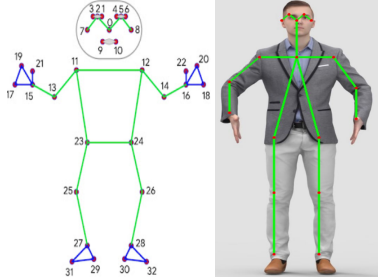
\includegraphics[width=0.6\linewidth]{assets/img-std.png}
	\caption{Пример оценки позы.}
	\label{img:std}
\end{figure}

\subsection{Категоризация для определения позы человека}

Способ классификации различных типов оценки позы основан на разрешении и количестве ориентиров, поскольку это отражает тип выполняемой оценки позы, то есть руки, лицо или тело.
Такой подход имеет смысл из-за свойств этих оценок, которые будут подчеркнуты при классификации ниже.

\begin{enumerate}[label=\arabic*)]

\item Низкое разрешение при наличии до 30 ориентиров. Если необходимо определить не так много ориентиров, то низкого разрешения будет достаточно для выполнения данной задачи. 
Это относится к оценке позы тела, поскольку в большинстве случаев имеется около 20 ориентиров, в то время как в некоторых случаях их немного больше 30, как показано в таблице \ref{table:standart}.
Кроме того, проблема наложения и сложных поз, которая широко распространена при оценке положения тела, решается с помощью большого <<рецепторного поля>> и не требует высокого разрешения, таким образом, для идентификации ориентиров достаточно низкого разрешения

\item Высокое разрешение для сложных поз.
При наличии более 30 ориентиров, которые являются крупными и сложными, для точной локализации требуется более высокое разрешение для их точной локализации.
Оценка позы лица обычно имеет 68 ориентиров \ref{table:standart}. Аналогично, при оценке позы руки требуется всего 42 ориентира \ref{table:standart}. Для того чтобы учесть большое количество и размер ориентиров, необходимо высокое разрешение.  

\end{enumerate}

\section{Наборы данных, используемых в определении позы человека}

Наборы данных являются важным аспектом в машинном обучении. Для того чтобы модели машинного обучения выполняли задачу, их алгоритмы должны быть сначала обучены, а затем протестированы, чтобы убедится, что они правильно интерпретируют данные для выполнения задачи.

Это делается с помощью наборов данных, которые состоят из обучающих и тестовых данных. 
Для каждого типа определения позы человека существует свой набор данных.

\subsection{Наборы данных по определению позы тела}

 
\begin{enumerate}[label=\arabic*)]
	
	\item COCO \cite{COCO}: это наиболее широко используемый двумерный набор данных тела, в первую очередь для определения позы нескольких людей.
	Хотя он используется для обнаружения объектов и содержит изображения, помогающие в этом, он содержит более 330 тыс. изображений и 200 тыс. людей, помеченных ориентиров до 17 по всему телу.
	Первый набор был выпущен в 2014 году, но с тех пор был изменен.
	Существет 2 версии наборов данных COCO для определения позы человека: ориентиры COCO 2016 и 2017 года, отличаются в разделении на обучение, проверку и тестировании.
	
	\item  MPII \cite{MPII}: этот набор данных двумерных тел используется в основном для оценки позы одного человека.
	Он содержит около 25 тысяч изображений, содержащих 40 тыс. человек с 16 вручную отмеченных суставов тела, это отличается от COCO, так как там отмечается 17 суставов тела.
	Изображения охватывают 410 различных видов человеческой деятельности, таких как танцы, бег, охота, и помечаются соответствующим видами деятельности.
	Каждое изображение было взято из видеоролика YouTube и были предоставлены предшествующие были предоставлены предшествующие и последующие кадры, которые не были отмечены, что является еще одним отличием от COCO. 
	Кроме того, были добавлены расширенные описания, такие как перекрытые части тела и трехмерная ориентация туловища и голова.
	Набор был сделан в 2014 году.
	
	\item AI Challenger Human Keypoint Detection \cite{AI_chlenger}: этот набор данных по двумерным телам является крупнейшим, когда речь идет о двухмерном описании положении человека.
	Он содержит более 300 тыс. отмеченных изображений высокого разрешения для обнаружения ориентиров (14 ориентиров на человека) и более 600 тыс. тестовых изображений.
	Все изображения были собраны из поисковых систем, и, как и в наборе данных MPII, сфокусированы на повседневной деятельности людей в различных позах.
	Разница в системе подбора изображений, и в дополнительных функциях: распознавание пустых снимков на основе атрибутов.
	Набор был сделан в 2017 году.
	
	\item PoseTrack \cite{PoseTrack}: это двумерный набор данных по телу на основе видео, который содержит около 1356 видео, 46 тыс. отмеченных видеокадров и 276 тыс. помеченных поз тела.
	Он в основном используется для оценки позы тела несколько людей, где каждый человек имеет уникальный идентификатор трека с отметок, включающими до 15 ключевых точек тела.
	PoseTrack отличается от других набор данных тела тем, что в нем используется видеозаписи вместо изображений и другое количество ключевых точек.
	Набор был сделан в 2017 году.
	
\end{enumerate}

\subsection{Наборы данных по определению направления головы}

\begin{enumerate}[label=\arabic*)]
	
	\item 300W \cite{300-W}: этот двумерный набор лиц является коллекцией нескольких других наборов данных, включая HELEN, AFW, LFPW и IBUG, которые были отмечены 68 ориентирами, что означает, что 300W тоже маркирует свои изображения с помощью 68 ориентиров.
	В общей сложности в нем общей сложности в нем имеется около 4000 учебных изображений и 600 тестовых изображений: 300 изображений лиц в помещении и 300 изображений лиц на улице.
	Все они имели различные условия съемки, такие как освещение, цвет, эмоции, размер лица, угол наклона и количество присутствующих лиц.
	Набор был сделан в 2013 году.
	
	\item AFLW \cite{AFLW}: этот набор двумерных лиц содержит около 25 тыс. изображений лиц, различающихся по внешнему виду, такому как как поза, пол, возраст, этническая принадлежность и выражение лица.
	Отличие этого набора в том, что он маркирован только 21 ориентиром и имеет больший угол съемки лица по сравнение 300W.
	Набор был сделан в 2011 году.
	
	\item COFW \cite{COFW}: этот набор данных двумерных лиц в основном ориентирован на маркировку изображений лиц, которые частично закрыты другими объектами или самим лицом.
	Состоит из около 1,3 тыс. учебных и 507 тестовых изображений, которые помечены 29 ориентирами, что он отличается от других наборов данных лиц.
	Набор сделан в 2013 году.
	
	\item WFLW \cite{WFLW}: этот двумерный набор лиц является одним из самых подробных наборов данных. 
	Он состоит из 7,5 тыс. учебных и 2,5 тыс. тестовых изображения, в частности, они широкий диапазон эмоций, поз, размытости и условий освещения.
	Кроме того, они маркированы с помощью 98 плотно привязанных ориентиров, что также отличает их от других наборов данных лиц.
	Набор данных собран в 2018 году. 
	
	
\end{enumerate}

\subsection{Наборы данных по определению позы руки}

\begin{enumerate}[label=\arabic*)]
	
	\item BigHand2.2M \cite{BigHand2.2M}: этот набор данных трехмерных рук является самым большим набором данных рук на сегодняшний день, поскольку содержит около 2,2 миллиона глубинных изображений отдельных рук с 21 ориентирами, полученных от 10 испытуемых.
	Варьирование положения испытуемых и ориентации рук помогло создать разнообразный набор точек зрения на руки.
	Набор данных разбит на 3 части: 1,5 миллиона по 13 кадров схематичными позами, которые охватывают все сочленения которые может свободно принять человеческая рука; 375 тыс. кадров случайных поз, которые показывают, как испытуемые используют свои руки для ориентации в пространстве; 290 тыс. кадров эгоцентрических поз, в которых испытуемые выполняют 32 экстремальные позы, которые представляют собой позы рук, где каждый палец принимает максимально согнутое или вытянутое положение, в сочетании со случайными движениями.
	Набор сделан в 2017 году.
	
	\item GANerated Hand Dataset \cite{GANeratedHands_CVPR2018}: это набор двумерных и трехмерных данных рук, содержащий 330 тыс. кадров, которые представляют собой синтезированне формы рук и имеют 21 ориентир.
	В отличие от BigHand2.2M, для захвата поз рук использовались искусственные объекты, удерживаемые руками.
	Набор создан в 2018 году. 
	
	\item NYU Hand \cite{tompson14tog}: этот набор данных трехмерных рук содержит более 72 тыс. кадров в обучающем наборе от одного испытуемого и более 8 тыс. кадров от двух разных испытуемых в тестовом наборе.
	По сравнению с другими наборами данных рук этот набор данных выделяется тем, что это снимки сделаны с помощью тепловизора. 
	Набор собран в 2014 году.
	
	\item HandNet \cite{WetzlerBMVC15}: этот набор данных трехмерных изображений рук является одним из самых больших набор данных по глубине.
	Он содержит 202 тыс. учебных и 10 тыс. тестовых кадров.
	В наборе присутствует 5 мужчин и 5 женщин для того, чтобы набор содержал разные размеры рук.
	Изображения были промаркированы 6 ориентирами.
	Набор собран в 2015 году.
	
	
\end{enumerate}

\section{Примеры использования определения позы человека}

Определение положения человека можно использовать во множестве областей. В данном разделе будут приведены некоторые из них.

\subsection{Личные тренеры на основе глубоко обучения}

Для поддержания физического здоровья было создано приложение Zenia \cite{Zenia} --- это приложение для занятия йогой на основе искусственного интеллекта, использующее определение позы человека.
Оно помогает принимать правильные позы при занятиях йогой.
Приложение использует камеру для распознавания позы и оценивает ее точность.

Также определение позы человека используется не только в йоге, но и в тяжелой атлетике, для предотвращения травм.

\subsection{Роботехника}

Еще одной из областей применения определения позы человека является роботехника.

Для обучения роботов используются глубокое обучение на основе моделей определения позы человека, так как это упрощает задачу программистам, которые пишут логику ходьбы для роботов. 

\subsection{Дополнительная реальность}

За недавний период быстрыми темпами начало развиваться дополнительная реальность и виртуальная реальность. Для данных направлений необходимо отслеживать движений человека. Как раз для отслеживания используются нейронные сети на основе определения позы человека.

\subsection{Распознавание поз спортсменов}

В наши дни во всех видов спорта вводится анализ данных и одним из ключевых направлений является определение позы спортсменов.

Распознавание позы спортсмена необходимо для обучения спортсменов, чтобы совершенствовать их технику и улучшать результаты. Для этой области используются нейронные сети на основе определения позы человека.